\RequirePackage{fix-cm}                                     % Fix font with siunitx
\documentclass[english, twocolumn]{article}                 % Document type
%\usepackage{emptypage}                                      % Empty pages
\RequirePackage[l2tabu, orthodox]{nag}                      % Detect deprecated packages, commands, etc.
\usepackage[all,error]{onlyamsmath}                         % Error on deprecated math commands like $$ $$.
\usepackage{algpseudocode}
\usepackage{algorithm}
\usepackage{listing}
\usepackage{graphics}
\AtBeginDocument{\catcode`$=3 }                             % Workaround for tikz
\usepackage{fixmath}                                        % Fix non ISO behaviour with capital greek letters
%\usepackage{refcheck}                                       % Display warning on unused references
%\ignoreunlbld                                               % Ignore equations in refcheck
\usepackage{todonotes}                                      % TODO

\usepackage{lipsum}                                         % Generate random text (ONLY FOR TEST PURPOSES)


% --- Mathematical packages ---
\usepackage{amsmath}                                        % Math
\usepackage{amsthm}                                         % Theorems and proofs
\usepackage{amssymb}                                        % Math symbols
\usepackage{bm}												% Bold math
\usepackage[per-mode=fraction,
            exponent-product=\cdot,
            separate-uncertainty=true,
            binary-units=true
           ]{siunitx}                                       % Physical units
%\usepackage{mathtools}                                      % Math tools


% --- Typographical packages ---
% - Bases -
\usepackage[utf8]{inputenc}                                 % UTF-8 Encoding
\usepackage[T1]{fontenc}                                    % Font encoding
\usepackage{babel}                                          % Translation
\usepackage[babel]{csquotes}                                % Quotes
\usepackage{comment}                                        % Comments
% - Font -
\usepackage{newtxtext,newtxmath}                            % Times font
\usepackage[toctitles,compact,explicit]{titlesec}           % Custom chapter headings
\usepackage{microtype}                                      % Typographical improvements
\usepackage{ellipsis}                                       % Whitespace correction
% - Shape -
\usepackage[hyphens]{url}                                   % Hyphens in URLs
\usepackage{varioref}
\usepackage[hidelinks]{hyperref}                                       % Clickable references
\usepackage[noabbrev,capitalise]{cleveref}
\usepackage[backend=biber,					% Backend
            bibencoding=utf8,				% File encoding (BibTex = ASCII, Biber = UTF8)
            bibstyle=authoryear,		    % Reference style
            citestyle=authoryear,           % Citation style
            bibwarn=true,                   % Enable warnings
            natbib=true,                    % Natbib compatibility
            style=alphabetic,
            maxcitenames=2,					% Cite : > 2 name = et al.
            maxbibnames=99,					% Bib  : show all names
            sortcites=true,					% Sorting
            block=space,					% Space between citations
            giveninits=true,				% Compress first names
            uniquename=init,				% Compatible with 'giveninits=true'
            isbn=false,                     % Disable ISBN
            doi=false                       % Disable DOI
           ]{biblatex}
\usepackage{fancyhdr}                                       % Custom head- and foot-lines
\usepackage{setspace}                                       % Spacing between lines
\usepackage[titles]{tocloft}                                % Spacing in table of contents
%\usepackage{abstract}                                       % Abstract
\usepackage[margin=2cm]{geometry}                                       % Geometry of a page

% --- Graphical packages ---
\usepackage{float}                                          % float environment settings
\usepackage{graphicx}                                       % Figures
\usepackage{caption}                                        % Figures and captions
\usepackage{subcaption}                                     % Figures and captions (side-by-side)
\usepackage{booktabs}                                       % Improved tables
\usepackage{multirow}                                       % Multirow


\usepackage{pbox}
% Disable underfull box warnings when breaking URLs
\usepackage{etoolbox}
\apptocmd{\sloppy}{\hbadness 10000\relax}{}{}

\bibliographystyle{alpha}
\addbibresource{refs.bib}

\setlength\columnsep{30pt}
\setlength\voffset{1cm}
\addtolength{\textheight}{-2cm}

\usepackage{chngcntr}
\usepackage{graphicx}
\usepackage{mathtools}
\usepackage{mdframed}
\usepackage{pgfplots}
\usepackage{csquotes}
\usepackage{float}
\usepackage{tikz}
\usetikzlibrary{intersections, positioning, calc, fit}

\usepackage{graphicx}
\graphicspath{{./media/}}

% from https://tex.stackexchange.com/questions/66216/draw-arc-in-tikz-when-center-of-circle-is-specified
\def\centerarc[#1](#2)(#3:#4:#5);%
%Syntax: [draw options] (center) (initial angle:final angle:radius)
    {
    %\draw[#1] ($(#2)+({#5*cos(#3)},{#5*sin(#3)})$) arc (#3:#4:#5);
    \draw[#1]([shift=(#3:#5)]#2) arc (#3:#4:#5);
    }

\DeclarePairedDelimiter\ceil{\lceil}{\rceil}
\DeclarePairedDelimiter\floor{\lfloor}{\rfloor}

\counterwithin*{section}{part}

\title{Wolken und Himmel dynamisch rendern}
\author{Jan Spindler, Simon Katz}

\newcommand{\matNr}{3338877, 3309821}
\newcommand{\reportType}{Project Group}
\date{\today}


% Generate author and title
\makeatletter

\begin{document}

{
  \twocolumn[
    \begin{center}
      \LARGE \reportType{}: \\ \@title
    \end{center}
    \begin{center}
      \large\@author \\
      \large Mat. Nr.: \matNr{}
    \end{center}
    \begin{center}
      \large \@date
    \end{center}
    \vspace{0.3cm}
    % \captionsetup{type=figure}
% 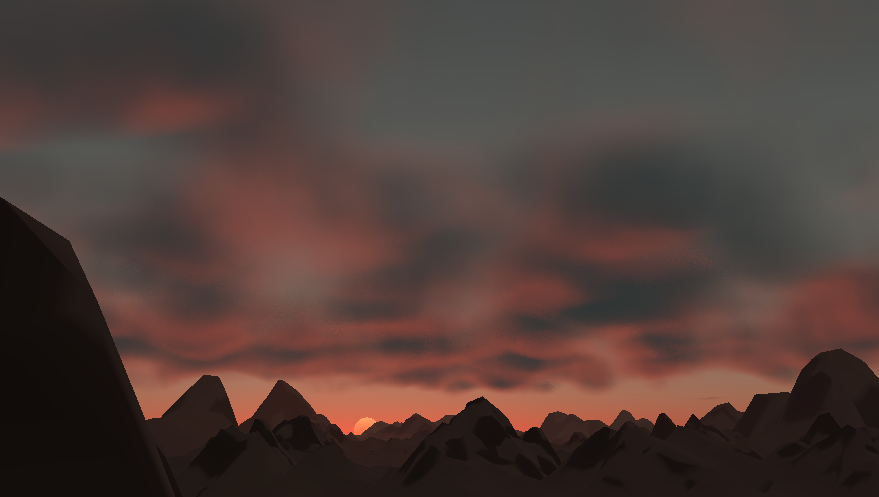
\includegraphics[width = \textwidth]{figures/teaser.png}
% \captionof{figure}{The robot as a means to put things on tables efficiently.}
% \label{fig:teaser}

    \vspace{0.8cm}
  ]
}

\section*{Abstract}
\label{sec:abstract}

Im folgenden stellen wir physikalisch basierte, dynamische Modelle für Wolken und Atmosphäre mit dem Ziel des
Echtzeitrenderings vor.

Ein physikalisch basierter Himmel trägt viel zu dem Realismus und der Stimmung einer gerenderten Szene bei. Wolken
müssen abhängig vom Wetter und die Atmosphäre je nach Sonnenstand und Partikeldichte (Smog in Städten, strahlend
blauer Himmel in der Karibik) ihr Aussehen ändern.

Aufgrund der Qualität unseres Modells ist es vielfältig Einsetzbar, von Videospielen über Architektur oder
Designanwendung bis hin zu mobile(re)n Einsatzbereichen wie VR/AR.


\part{Wolken}
\section{Einleitung}
\label{sec:introduction}

Wolken sind in der Realität maßgeblich für die Dynamik, Stimmung und Lichtverhältnisse des Alltags. Es liegt also nahe, dass Wolken einer gerenderten Szene mehr Realismus verleihen können. Die korrekte Wechselwirkung von Wolken und Licht ist sehr komplex und kann nur mit viel Rechenkapazität und Zeit simuliert werden. Wir möchten in diesem Part ein Verfahren und dessen Grundlagen darlegen, welches durch Vereinfachung physikalischer Modelle Wolken in Echtzeit rendern kann.\\

Im Folgenden werden drei verschiedene Ansätze zum Rendern von Wolken kurz vorgestellt.

Ein simpler Ansatz zum Rendern von Wolken ist das Verwenden von Skyboxen. Die Wolken und der Himmel sind dabei statisch und werden in einer CubeMap gespeichert. Da diese Technik leicht und billig umzusetzen ist, wird sie auch in modernen Anwendungen verwendet.

In der Arbeit Deep Scattering: Rendering Atmospheric Clouds with Radiance-Predicting Neural Networks von Kallweit et al. \cite{Kallweit17} wird ein Radianz vorhersagendes Neuronales Netzwerk antrainiert, um realistische Wolken innerhalb von wenigen Minuten bis Sekunden zu rendern.

In seiner Master These Convincing Cloud Rendering stellt Högfeldt \cite{Högfeldt16} einen Ansatz vor, mit dem in Echtzeit dynamische und realistische Wolken gerendert werden können. Dieser Ansatz ist durch die Technik von Schneider und Vos \cite{Schneider15} inspiriert und wurde zusammen mit den Entwicklern von Frostbite in einem Modul für die Frostbite Engine umgesetzt. Wir greifen die Methoden von Högfeldt auf, um einen Echtzeit Wolkenrenderer zu implementieren.\\

Diese Arbeit strukturiert sich wie folgt. Zunächst wird auf die Grundlagen von Wolken und ihrer Interaktion mit der Umwelt eingegangen. Im darauf folgenden Abschnitt werden die nötigen Methoden dargelegt, die es ermöglichen einen Wolkenrenderer zu implementieren. Danach werden die spezifische Implementierung der Methoden und die Parameter zur Steuerung der Methoden so wie Optimierungen näher erläutert. Diese Parameter und Optimierungen werden anschließend im Bezug auf visuelle Qualität und Performanz ausgewertet. Anhand dieser Auswertung werden Parameterkombinationen ermittelt, um bekannte realistische Wolkenformationen zu rendern.

Die Ergebnisse aus Sektion \ref{sec:evaluation} zeigen, dass es gelingt realistische Wolken in Echtzeit auf acht Jahre alter Grafikhardware zu rendern. Der Wolkenrenderer bietet sich somit für eine Implementierung in Echtzeitanwendungen wie Videospiele oder Designsoftware an. Darüberhinaus kann der Ansatz speziell im Bezug auf Wechselwirkung mit Geometrie weiterentwickelt werden, um mehr Realismus und Dynamik in eine Szene zu bringen.

\section{Wolkenmodelle}
\label{sec:model}

\subsection{Varianten}
Wolken können in verschiedenen Varianten auftreten \cite{Högfeldt16}. Diese unterscheiden sich in Form, Höhe und Niederschlag. Die Namen von Wolken setzen sich oft aus einer Kombination ihrer Attribute zusammen. Die Höhe einer Wolke wird durch die Attribute Cirrus für hoch und Alto für mittelhoch angegeben. Andere Attribute wie Cumulus für geschwollene Wolken oder Stratus für geschichtete Wolken geben die Form an. Das Attribut Nimbus beschreibt Wolken mit Niederschlag.

Zu bekannten Wolkenarten gehören Stratus (niedrig, ebene Schichten), Cirrus (hoch, dünne Streifen) und Cimulus (einzelne Haufen).

\subsection{Beleuchtung}
Wolken bestehen aus Ansammlungen von Wasserpartikeln. Um realistische Wolken rendern zu können, müssen wir verstehen, wie Licht mit diesen Wasserpartikeln interagiert. Dieser Abschnitt folgt der Arbeit von Högfeldt \cite{Högfeldt16} und geht auf vier verschiedene Arten ein, auf die Photonen mit den Wasserpartikeln wechselwirken. Diese vier Varianten sind Absorbtion, In-Scattering, Out-Scattering und Emission. Ziel ist es, diese Wechselwirkung in ein mathematisches Modell einzupflegen, das für einen Renderer verwendet werden kann.

\subsubsection{Absorbtion}
Bei Absorbtion wird ein Photon durch das Medium aufgenommen und in eine andere Energieform wie Wärme umgewandelt. Dies führt zu einem Verlust der Radianz, der durch Gleichung \ref{eq:absorbtion} beschrieben wird. Der Absorbtionskoeffizient $ \sigma_a $ gibt die Wahrscheinlichkeit an, dass ein Photon von dem Medium absorbiert wird.

\begin{equation}
    L_a(x, \vec{\omega}) = e^{-\sigma_a(x)dt} L(x, \vec{\omega})
    \label{eq:absorbtion}
\end{equation}

\subsubsection{Streuung}
Beim Wechselwirken mit einem Medium können Photonen in verschiedene Richtungen gestreut werden. Dabei kann sich die Radianz durch einfallende Photonen aus anderen Richtungen erhöhen (In-Scattering) oder durch das Streuen von Photonen in andere Richtungen reduzieren (Out-Scattering). Der Streuungskoeffizient $ \sigma_s $ gibt die Wahrscheinlichkeit an, dass ein Photon durch das Medium gestreut wird. $ P(x, \vec{\omega}) $ ist eine Phasenfunktion, welche einer Richtung die Wahrscheinlichkeit zuordnet, dass in diese gestreut wird. Das Erhöhen der Radianz durch ein Photon, das aus einer anderen Richtung einfällt wird durch Gleichung \ref{eq:in-scatter} beschrieben.

\begin{multline}
    L_{s-in} = \sigma_s(x) L_i(x, \vec{\omega})\\
    L_i(x, \vec{\omega}) = \int_{\Omega 4 \pi}^{}P(x, \vec{\omega}) L(x, \vec{\omega}) d\vec{\omega}\\
    \label{eq:in-scatter}
\end{multline}

\subsubsection{Auslöschung}
Die Wahrscheinlichkeit, dass ein Photon mit dem Medium durch Absorbtion oder Streuung in einer andere Richtung wechselwirkt und somit zu einer reduzierten Radianz führt, ist durch den Koeffizienten $ \sigma_e $ als Summe der Streuungs- und Auslöschungswahrscheinlichkeiten gegeben. Diesen Zusammenhang zeigt Gleichung \ref{eq:extinction}.

\begin{equation}
    \sigma_e = \sigma_a + \sigma_s
    \label{eq:extinction}
\end{equation}

Die Transmittance gibt an, wie viele Photonen ungestört von dem Punkt $ x_0 $ zu dem Punkt $ x_1 $ durch das Medium traversieren können. Gleichung \ref{eq:transmittance} zeigt, wie diese sich mittels dem Lambert-Beer’schen Gesetz aus dem Koeffizienten $ \sigma_e $ berechnen lässt.

\begin{equation}
    T_r(x_0, x_1) = e^{-\int_{x_0}^{x_1} \sigma_e(x) dx}
    \label{eq:transmittance}
\end{equation}

\subsubsection{Emission}
Bei der Emission kommt es zu einer Erhöhung der Radianz $ L_e(x, \vec{\omega}) $, weil andere Energieformen in Licht umgewandelt werden. Im Rahmen dieser Arbeit vernachlässigen wir die Emission, die durch andere Energieformen ausgelöst werden kann.

\subsubsection{Strahlungstransportfunktion}
Durch Kombination der Besprochenen Interaktionen zwischen Licht und dem Medium, lässt sich die Gleichung \ref{eq:radiative-transfer} durch Energieerhaltung herleiten \cite{Högfeldt16}. Diese beschreibt die Radianz an der Position $ x $ entlang eines Strahls mit Richtung $ \vec{\omega} $.

\begin{multline}
    L(x, \vec{\omega}) =
    T_r(x, x_s) L(x_s, -\vec{\omega}) +\\
    \int_{0}^{s} T_r(x, x_t) L_e(x_t, -\vec{\omega}) dt +\\
    \int_{0}^{s} T_r(x, x_t) \sigma_s(x_t) L_i(x_t, -\vec{\omega}) dt\\
    \label{eq:radiative-transfer}
\end{multline}

\section{Methodik}
\label{sec:method}

\subsection{Ray Marching}
Da Wolken keine klar definierte Oberfläche haben wie andere 3D-Modelle, nutzen wir Ray Marching, um ein Volumen zu schneiden, in dem die Wolken gerendert werden. Für jeden Pixel wird der Ein- und Austritt eines Strahls mit dem Volumen berechnet. Zwischen dem Ein- und Austritt werden N sogenannte Primär Samples in gleichmäßigen Abständen berechnet. Für jedes dieser Primär Samples werden M Sekundär Samples in exponentiellen Abständen in Richtung Lichtquelle (Sonne) berechnet.

\subsection{Texturgenerierung}
Die in der vorangegangenen Sektion \ref{sec:model} beschriebenen Wahrscheinlichkeiten $ \sigma_a(x) $, $ \sigma_s(x) $ und $ \sigma_e(x) $ sind abhängig von der Dichte an der Position $ x $, da bei einer höheren Dichte mit mehr Partikeln interagiert werden kann. Somit ist das Aussehen der Wolken wesentlich davon abhängig, wie die Dichte in dem Volumen verteilt ist. Um eine realistische Dichteverteilung und somit realistische Wolken zu erhalten, wird eine Kombination aus 3 Texturen genutzt \cite{Högfeldt16}. Wie diese generiert werden können, wird im Folgenden erläutert.

\subsubsection{Noise}
Um Texturen zu generieren, die zu einer möglichst natürlichen Dichteverteilung kombiniert werden sollen,
werden Perlin und Worley Noise genutzt.

Zur Generierung von Perlin Noise \cite{Perlin85} werden in einem Gitter Pseudozufällige Gradienten verteilt. Der Wert des Perlin Noises an einem Punkt $ x $ errechnet sich durch Interpolation der zu $ x $ benachbarten Gradienten.

Um Worley Noise zu generieren, werden in einer Fläche oder in einem Volumen zufällige Punkte verteilt. Der Wert des Worley Noises errechnet sich dann durch den kleinsten Abstand zu einem der generierten Punkte. Um eine Gleichverteilung der Werte sicherzustellen, kann das Volumen in ein Gitter unterteilt werden, in dem pro Teilvolumen nur ein Punkt generiert wird.

Perlin und Worley Noise werden in Abbildung \ref{fig:noise} veranschaulicht.

\begin{figure}[H]
    \centering
    \subfloat[\centering Perlin]{{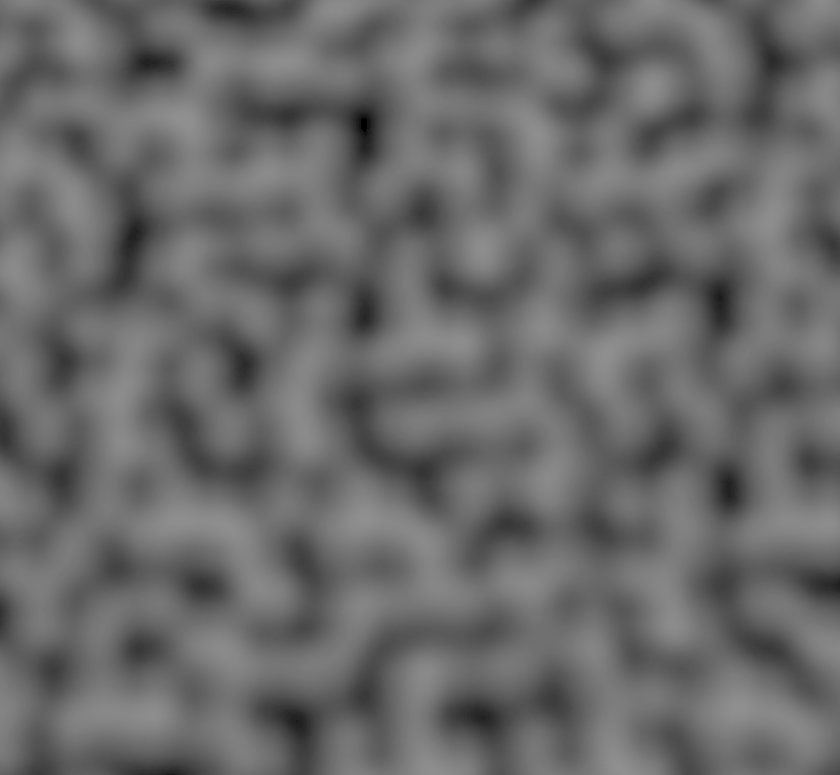
\includegraphics[width=3cm]{media/perlin.png} }}%
    \qquad
    \subfloat[\centering Worley]{{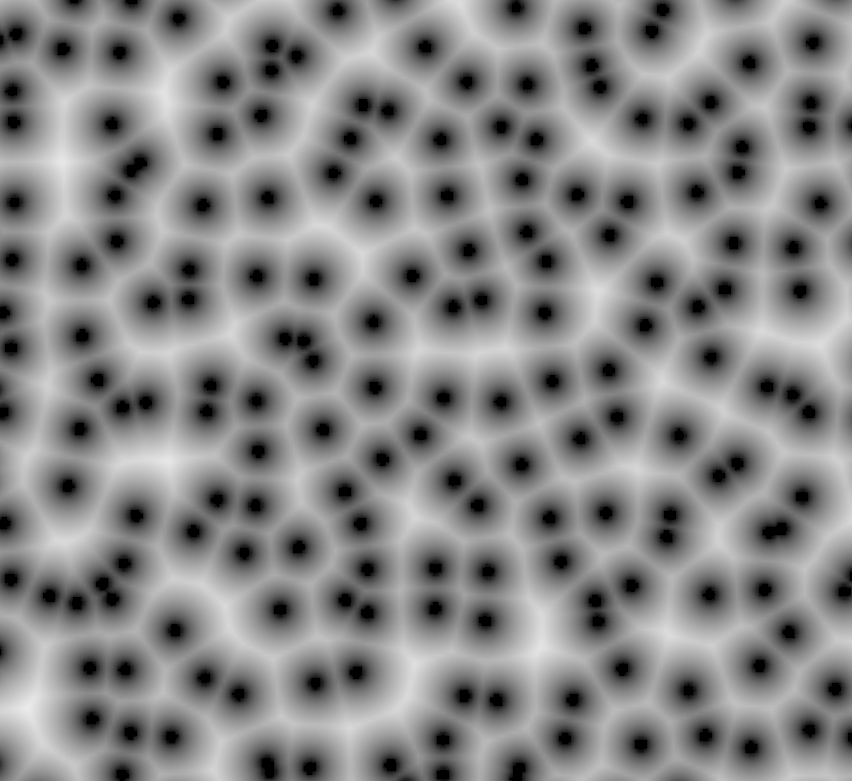
\includegraphics[width=3cm]{media/worley.png} }}%
    \caption{Perlin und Worley Noise}
    \label{fig:noise}
\end{figure}

\subsubsection{Shape Textur}
Die erste dieser drei Texturen ist die dreidimensionale Shape Textur. Sie besteht aus einem Perlin Kanal und drei Worley Kanälen mit unterschiedlichen Oktaven. Gleichung \ref{eq:shape} zeigt, wie der $ shape $ Wert aus der Textur berechnet wird.

\begin{equation}
    shape = perlin \cdot (worley_0 + worley_1 + worley_2)
    \label{eq:shape}
\end{equation}

\subsubsection{Detail Textur}
Die Detail Textur ist wie die Shape Textur dreidimensional. Sie besteht aus drei Worley Kanälen mit unterschiedlichen Oktaven. Der $ detail $ Wert wird aus dieser Textur wie in Gleichung \ref{eq:detail} berechnet.

\begin{equation}
    detail = \frac{1}{3} (worley_0 + worley_1 + worley_2)
    \label{eq:detail}
\end{equation}

\subsubsection{Weather Textur}
Die Weather Textur ist zweidimensional und besteht aus den drei Kanälen Coverage, Height und Altitude. Diese Kanäle bestimmen eine Dichte, die mit $ shape $ und $ detail $ angepasst werden. In unserer Implementierung wird die Weather Textur auch durch eine Kombination aus Worley und Perlin Noise berechnet. Um noch realistischere Wolken zu simulieren, kann die Weather Textur mit echten Wolkendaten gefüllt werden.

\subsection{Dichte Berechnung}
Algorithmus \ref{alg:density} zeigt, wie die Shape, Detail und Weather Texturen kombiniert werden, um die Dichte zu berechnen.

\begin{algorithm}[H]
\caption{Berechnung der Dichte \cite{Högfeldt16}}
\label{alg:density}
\begin{algorithmic}[1]
\State $ (cov, hei, alt) \gets weather(pos.xz) $
\State $ density \gets cov $
\State $ density \gets density \cdot heightSignal(hei, alt, pos.y) $
\State $ density \gets density \cdot shape(pos) $
\State $ density \gets density - detail(pos) $
\State $ density \gets density \cdot heightGradient(hei, alt, pos.y) $
\end{algorithmic}
\end{algorithm}

\subsubsection{Height Signal}
Das Height Signal verändert die Dichte in Abhängigkeit von der Höhe des Sample Punktes \cite{Högfeldt16}, so dass die Wolke vertikal auf das Intervall $ [altitude, altitude + height] $ begrenzt ist. Dabei soll die Dichte in der Mitte am höchsten und an den Rändern des Intervalls $ 0 $ sein. Diesen Effekt realisiert die Funktion aus Gleichung \ref{eq:height_signal}.

\begin{equation}
\label{eq:height_signal}
    heightSignal(h, a, y) = (y - a) (y - a - h) \frac{-4}{h^2}
\end{equation}

\subsubsection{Height Gradient}
Der Height Gradient ist ein linear steigender Gradient auf dem Intervall $ [altitude, altitude + height] $ \cite{Högfeldt16}. In Abhängigkeit von der Höhe des Sample Punktes wird ein Faktor zwischen $ min $ und $ max $ zurückgegeben. Diesen Zusammenhang verdeutlicht Gleichung \ref{eq:height_gradient}.

\begin{equation}
\label{eq:height_gradient}
    heightGradient(h, a, y) = lerp(min, max, \frac{y - a}{h})
\end{equation}

\subsection{Beleuchtung}
Für unseren Ansatz vereinfachen wir die Strahlungstransferfunktion aus Gleichung \ref{eq:radiative-transfer} zu der Gleichung \ref{eq:simple_rendering} \cite{Högfeldt16}.

\begin{equation}
\label{eq:simple_rendering}
    L_(x, \vec{\omega}) = \int_{0}^{s} T_r(x, x_t) \sigma_s(x_t) L_i(x_t, -\vec{\omega}) dt
\end{equation}

Algrorithmus \ref{alg:lighting} approximiert Gleichung \ref{eq:simple_rendering} durch Summierung an den Primär Samples. $ stepSize $ beschreibt hier den Abstand zwischen zwei aufeinanderfolgenden Primär Samples.

\begin{algorithm}[H]
\caption{Beleuchtung \cite{Högfeldt16}}
\label{alg:lighting}
\begin{algorithmic}[1]
\State $ scatteredLight \gets vec3(0.0) $
\State $ transmittance \gets 1.0 $
\For{$ pos \in primarySamples $}
    \State $ sampleSigmaS \gets sigmaS \cdot density(pos) $
    \State $ sampleSigmaE \gets sigmaE \cdot density(pos) $
    \State $ ambient \gets ambientGradient \cdot ambientColor $
    \State $ S \gets (evalLight(pos, -lightDir) \cdot phase + ambient) \cdot sampleSigmaS $
    \State $ T_r \gets e^{-sampleSigmaE \cdot stepSize} $
    \State $ S_{int} \gets \frac{S - S \cdot T_r}{sampleSigmaE} $
    \State $ scatteredLight \gets transmittance \cdot S_{int} $
    \State $ transmittance \gets transmittance \cdot T_r $
\EndFor
\end{algorithmic}
\end{algorithm}

\subsubsection{Inter- und Intracloud Schatten}
Die Funktion $ evalLight(pos, dir) $ wertet aus, wie viel Licht von der Sonne die Position $ pos $ aus der Richtung $ dir $ erreicht. Dazu bilden wir den Strahl von $ pos $ in Richtung $ dir $ zum Rand des Volumens $ x_0 $. Wir schätzen das Licht das $ pos $ erreicht durch die Transmittance entlang dieses Strahls.

\begin{figure}[H]
    \centering
    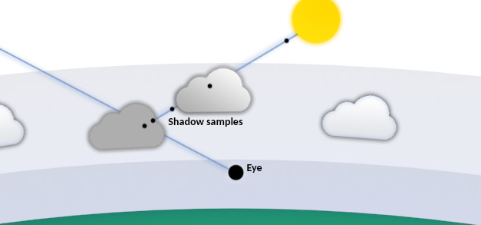
\includegraphics[width=8cm]{media/cloud-shadow.png}
    \caption{Inter- und Intracloud Schatten \cite{Högfeldt16}}
    \label{fig:shadow}
\end{figure}

Wir approximieren das Integral $ T_r(x_0, pos) $ durch eine Summe über den Sekundär Samples, wie in Algorithmus \ref{alg:second_lighting} beschrieben ist. Abbildung \ref{fig:shadow} zeigt die Sekundär Samples entlang des Strahls in exponentiellen Abständen.

\begin{algorithm}[H]
\caption{Inter- und Intracloud Schatten}
\label{alg:second_lighting}
\begin{algorithmic}[1]
\State $ transmittance \gets 1.0 $
\For{$ pos \in secondarySamples $}
    \State $ sampleSigmaE \gets sigmaE \cdot density(pos) $
    \State $ T_r \gets e^{-sampleSigmaE \cdot stepSize} $
    \State $ transmittance \gets transmittance \cdot T_r $
\EndFor
\end{algorithmic}
\end{algorithm}

\subsubsection{Phasenfunktion}
Der $ phase $ Parameter aus Algorithmus \ref{alg:lighting} wird durch die Henyey-Greenstein Phasenfunktion \cite{Henyey41} aus Gleichung \ref{eq:phase} berechnet.

\begin{equation}
\label{eq:phase}
    p_{HG}(\theta) = \frac{1 - g^2}{4\pi (1 + g^2 - 2g \cdot cos(\theta))^{1.5}}
\end{equation}

$ \theta $ ist der Winkel zwischen der Richtung zur Kamera und der Richtung des Lichts.

\subsubsection{Ambient}
Der Ambient Gradient aus Algorithmus \ref{alg:lighting} ist wie der Height Gradient der Dichteberechnung ein linearer Gradient auf der Höhe innerhalb einer Wolke. Dieser skaliert den Einfluss des Umgebungslichts.

\section{Implementierung}
\label{sec:implement}

\subsection{Volumen}
In der Arbeit von Högfeldt \cite{Högfeldt16} werden Volumen Ein- und Austritt berechnet, indem der Strahl mit zwei verschiedenen Kreisen mit unterschiedlichem Radius geschnitten wird. Dies führt zu einem gewölbten Horizont. In unserer Implementierung werden die Wolken in einem Quader gerendert. Die Schnittpunktberechnung mit dem Quader erfolgt über Ray Marching mit einer Box-SDF.

\subsection{Textur Generierung}
Die in Sektion \ref{sec:method} besprochenen Shape, Detail und Weather Texturen werden beim Start der Anwendung vorberechnet. Perlin Noise wird durch eine Funktion der Bibliothek GLM generiert. Worley Noise wird von einem Computeshader berechnet, um die Ladezeit zu verkürzen. Die Shape Textur hat 128 x 32 x 128 Einträge, die Detail Textur hat $ 32^3 $ Einträge und die Weather Textur hat $ 256^2 $ Einträge. Die Größen der Shape und Detail Texturen wurden von Högfeldt \cite{Högfeldt16} übernommen.

\subsection{Kombinieren mit Geometrie}
Da die Wolken keine eindeutige Tiefe haben, kann kein gewöhnlicher Tiefentest zwischen Wolken und Geometrie angewendet werden. Um den Zusammenhang zwischen Geometrie und Wolken korrekt abzubilden, werden Primär Samples hinter der Geometrie verworfen. Dazu wird in jedem Schleifendurchlauf aus Algorithmus \ref{alg:lighting} die Tiefe des Sample Punktes mit der Tiefe der Geometrie verglichen. Das Colorblending wird dann zwischen der Geometrie und dem Ergebnis der Primär Samples vor der Geometrie ausgeführt. Die Colorblendingfaktoren sind $ 1.0 $ für die Wolkenfarbe und die Transmittance aus Algorithmus \ref{alg:lighting} für die Geometriefarbe.

\subsection{Wind}
Wolken werden durch Wind in der Atmosphäre bewegt. Wir simulieren Wind durch einen Offset in der Weather Textur \cite{Högfeldt16}.

\subsection{Parameter}
Durch das Einstellen von verschiedenen Parametern können unterschiedliche Varianten von Wolken gerendert und die Performanz des Systems beeinflusst werden. Der folgende Abschnitt stellt diese Parameter und ihre Effekte dar.

\subsubsection{Volumen}
Das Volumen mit dem die Strahlen geschnitten werden kann verschoben und skaliert werden.

\subsubsection{Dichte}
Die Samplingrate der Shape und Detail Texturen kann ge ändert werden um feinere oder gröbere Wolken darzustellen. Der Detailwert lässt sich weiter durch einen Schwellwert und einen Faktor einstellen. Der Detailwert wird nur von der Dichte subtrahiert, wenn die Dichte unter dem Schwellwert ist. Vor dem Subtrahieren wird der Detailwert mit dem Detailfaktor skaliert \cite{Högfeldt16}.

\subsubsection{Beleuchtung}
Für den Height Gradient der Dichteberechnung und den Ambient Gradient aus Algorithmus \ref{alg:lighting} können die minimalen und maximalen Werte eingestellt werden. Mit diesen Gradienten ist das Einstellen der Dichte und Helligkeit von Wolken möglich. So lassen sich Wolken mit und ohne Niederschlag darstellen \cite{Högfeldt16}. Der Faktor g aus der Henyey-Greenstein Phasenfunktion kann eingestellt werden, um das Streuungsverhalten zu verändern. $ \sigma_s $ und $ \sigma_E $ aus dem Algorithmus \ref{alg:lighting} können eingestellt werden.

\subsubsection{Sample Anzahl}
Da wir Gleichung \ref{eq:simple_rendering} durch eine Summe an diskreten Sample Punkten approximieren, hängt die Qualität der gerenderten Wolken wesentlich von der Anzahl an Primär und Sekundär Samples ab. Welchen Einfluss die Anzahl der Samples auf die visuelle Qualität und Performanz hat, wird in Sektion \ref{sec:evaluation} anhand mehrerer Messungen veranschaulicht.

Die Anzahl der Samples kann auch zur Laufzeit geändert werden. Die Sample Punkte werden im Shader in einem Array verwaltet. Da die Größe des Arrays nicht dynamisch gewählt werden kann, muss bei einer neuen Sample Anzahl die Pipeline mittels Specialization Constants neu erstellt werden.

\subsection{Optimierung}
Dieser Abschnitt geht auf mehrere Möglichkeiten ein, die visuelle Qualität und die Performanz des Renderers zu verbessern.

\subsubsection{Render Target Größe}
Eine Möglichkeit die Performanz bei gleichbleibender Sample Anzahl zu erhöhen, ist die Wahl eines kleineren Render Targets \cite{Högfeldt16}.

\subsubsection{Jittering}
Beim Samplen aus den Dichte Texturen kann es zu Aliasing Artefakten kommen, wie Abbildung \ref{fig:jittering} zeigt. Diese Artefakte lassen sich auf verschiedene Weisen reduzieren. Eine Option ist die Abtastungfrequenz zu erhöhen, indem mehr Primär Samples genutzt werden. Somit wird die visuelle Qualität gegen Performanz getauscht.

Eine sparsamere Methode ist das Nutzen von Jittering. Dabei wird für jeden Pixel ein zufälliger Offset berechnet, der die Primär Samples des Pixels verschiebt. Wie Abbildung \ref{fig:jittering} zeigt, reduziert Jittering effektiv die Artefakte und zeigt stattdessen ein Rauschen. Um dieses Rauschen zu entfernen, kann wieder die Primär Sample Anzahl erhöht werden. Bei geringem lokalen Kontrast fällt das Rauschen weniger auf. Das Jittering lässt sich mit einem Faktor $ j \in [0, 1] $ steuern. So kann zwischen Rausch- und Aliasingartefakten interpoliert werden.

\subsubsection{Low Transmittance Early Exit}
Liegen vor einem Primär Sample $ P_n $ viele Primär Samples mit einer hohen Dichte und somit einem hohen Einfluss auf das Ergebnis, ist der Einfluss des Samples $ P_n $ gering. Dieser Zusammenhang wird von Högfeldt \cite{Högfeldt16} ausgenutzt. Beim Low Transmittance Early Exit wird die Schleife aus Algorithmus \ref{alg:lighting} vorzeitig beendet, wenn die Transmittance einen Schwellwert unterschreitet. So können Samples mit geringem Einfluss verworfen werden. In Abbildung \ref{fig:low-early-exit} sind die Stellen rot makiert, an denen Low Transmittance Early Exit mit einem Schwellwert von $ 0.01 $ verwendet wurde.

\begin{figure}[H]
    \centering
    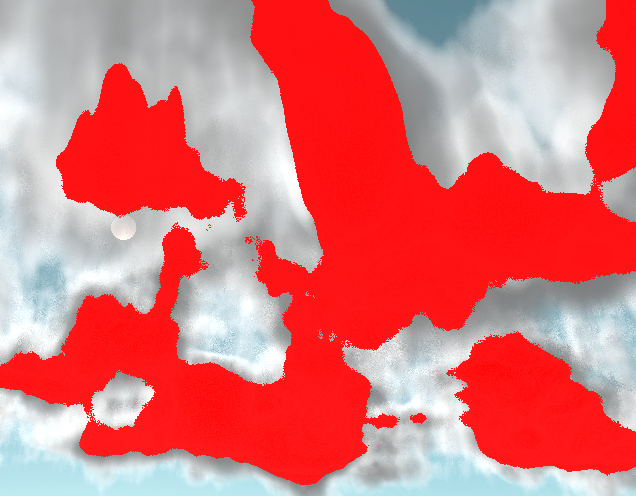
\includegraphics[width=8cm]{media/early-exit.png}
    \caption{Low Transmittance Early Exit in Rot}
    \label{fig:low-early-exit}
\end{figure}

\subsubsection{Temporal Upsampling}
Eine weitere Optimierung, die Högfeldt \cite{Högfeldt16} vorschlägt, ist das Temporal Upsampling. Dabei wird die Position eines Pixels $ P $ in dem letzten Bild ermittelt, um mit diesem zu interpolieren. Temporal Upsampling wurde zum Zeitpunkt der Einreichung unserer Arbeit noch nicht in den Renderer implementiert. Die Ergebnisse von Högfeldt aus Abbildung \ref{fig:temporal-upsampling} zeigen ein effektives Unterdrücken von Artefakten.

\begin{figure}[H]
    \centering
    \subfloat[Ohne Temporal Upsampling]{{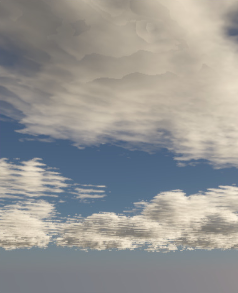
\includegraphics[height=4cm]{media/tu-left.png} }}%
    \qquad
    \subfloat[Mit Temporal Upsampling]{{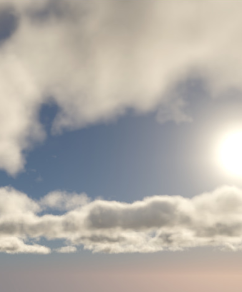
\includegraphics[height=4cm]{media/tu-right.png} }}%
    \caption{Temporal Upsampling visueller Vergleich \cite{Högfeldt16}}
    \label{fig:temporal-upsampling}
\end{figure}

\subsubsection{High Transmittance Early Exit}
Aufbauend auf den Methoden des Temporal Upsampling kann geprüft werden, ob ein Pixel in dem letzten Bild eine hohe Transmittance hatte. Ein hohe Transmittance kann als Abwesenheit von Wolken entlang des Strahls gedeutet werden. So lassen sich Pixel verwerfen, die wahrscheinlich keine Wolken darstellen.

\begin{figure}[H]
    \centering
    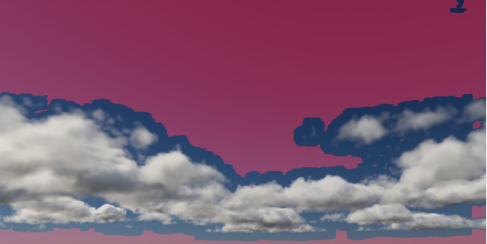
\includegraphics[width=8cm]{media/htee.png}
    \caption{High Transmittance Early Exit in Rot \cite{Högfeldt16}}
    \label{fig:htee}
\end{figure}

Wie in dem Ergebnis von Högfeldt \cite{Högfeldt16} auf Abbildung \ref{fig:htee} zu sehen ist, kann durch High Transmittance Early Exit eine große Anzahl an Pixeln verworfen werden.

\section{Evaluation}
\label{sec:evaluation}
In dieser Sektion wird die visuelle Qualität und die Performanz des Renderers unter verschiedenen Parameterbelegungen gemessen. Ziel dieser Messung ist eine Parameterempfehlung, die ein Gleichgewicht aus Qualität und Performanz bietet.

\subsection{Visuelle Ergebnisse}
Dieser Abschnitt beschäftigt sich mit den Auswirkungen der verschiedenen Parameter auf die visuelle Qualität der Wolken. Falls nicht explizit genannt sind die Parameter wie folgt belegt.\\

\begin{enumerate}
    \item Jittering $ = 1.0 $
    \item Primär Sample Anzahl $ = 40 $
    \item Sekundär Sample Anzahl $ = 3 $
    \item Detail Schwellwert $ = 0.3 $
    \item Detailfaktor $ = 0.35 $
    \item Low Transmittance Early Exit bei $ 0.01 $
\end{enumerate}

\subsubsection{Jittering}
Die Bilder aus Abbildung \ref{fig:jittering} zeigen das Ergebnis der Jitteringfaktoren $ 0.0 $, $ 0.33 $, $ 0.66 $ und $ 1.0 $ in der Reihenfolge links nach rechts und oben nach unten.

\begin{figure}[H]
    \centering
    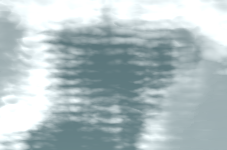
\includegraphics[width=4cm, height=3cm]{media/jittering_0.0.png}
    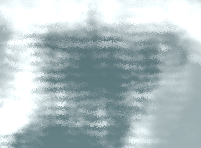
\includegraphics[width=4cm, height=3cm]{media/jittering_0.33.png}
    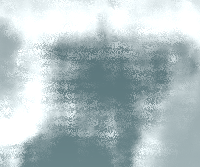
\includegraphics[width=4cm, height=3cm]{media/jittering_0.66.png}
    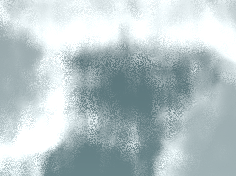
\includegraphics[width=4cm, height=3cm]{media/jittering_1.0.png}
    \caption{Jittering Faktor - 0.0, 0.33, 0.66, 1.0}
    \label{fig:jittering}
\end{figure}

\subsubsection{Primär Sample Anzahl}
Die Bilder aus Abbildung \ref{fig:1st-sample} zeigen das Ergebnis in Abhängigkeit von der Anzahl an Primär Samples in der Reihenfolge links nach rechts und oben nach unten.

\begin{figure}[H]
    \centering
    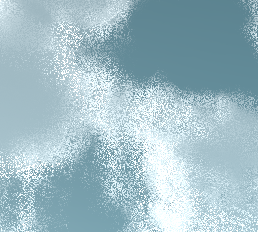
\includegraphics[width=4cm, height=3cm]{media/1st-sample-16.png}
    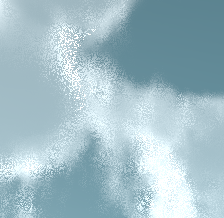
\includegraphics[width=4cm, height=3cm]{media/1st-sample-32.png}
    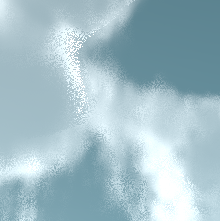
\includegraphics[width=4cm, height=3cm]{media/1st-sample-48.png}
    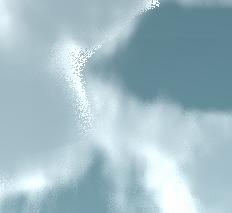
\includegraphics[width=4cm, height=3cm]{media/1st-sample-64.png}
    \caption{Primär Sample - 16, 32, 48, 64}
    \label{fig:1st-sample}
\end{figure}

\subsubsection{Sekundär Sample Anzahl}
Die Bilder aus Abbildung \ref{fig:2nd-sample} zeigen das Ergebnis in Abhängigkeit von der Anzahl an Sekundär Samples in der Reihenfolge links nach rechts und oben nach unten.

\begin{figure}[H]
    \centering
    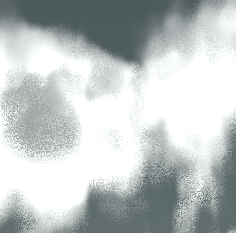
\includegraphics[width=4cm, height=3cm]{media/2nd-sample-2.png}
    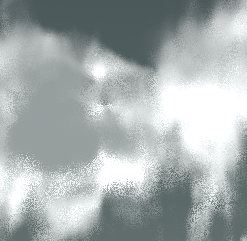
\includegraphics[width=4cm, height=3cm]{media/2nd-sample-3.png}
    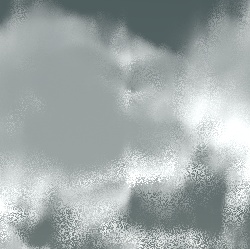
\includegraphics[width=4cm, height=3cm]{media/2nd-sample-4.png}
    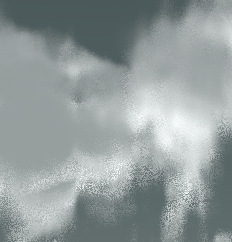
\includegraphics[width=4cm, height=3cm]{media/2nd-sample-5.png}
    \caption{Sekundär Sample - 2, 3, 4, 5}
    \label{fig:2nd-sample}
\end{figure}

\subsubsection{Detail Schwellwert}
Abbildung \ref{fig:detail-threshold} zeigt das Ergebnis bei unterschiedlichen Detail Schwellwerten in der Reihenfolge links nach rechts und oben nach unten.

\begin{figure}[H]
    \centering
    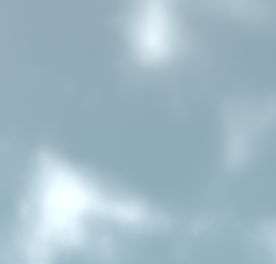
\includegraphics[width=4cm, height=3cm]{media/detail-threshold-0.0.png}
    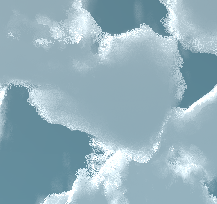
\includegraphics[width=4cm, height=3cm]{media/detail-threshold-0.1.png}
    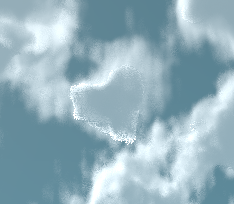
\includegraphics[width=4cm, height=3cm]{media/detail-threshold-0.2.png}
    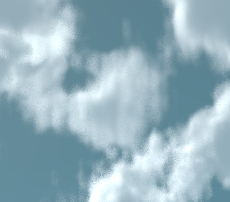
\includegraphics[width=4cm, height=3cm]{media/detail-threshold-0.3.png}
    \caption{Detail Schwellwert - 0.0, 0.1, 0.2, 0.3}
    \label{fig:detail-threshold}
\end{figure}

\subsubsection{Detailfaktor}
Abbildung \ref{fig:detail-factor} zeigt das Ergebnis bei unterschiedlichen Detailfaktoren in der Reihenfolge links nach rechts und oben nach unten.

\begin{figure}[H]
    \centering
    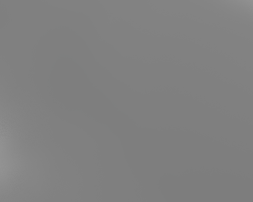
\includegraphics[width=4cm, height=3cm]{media/detail-factor-0.0.png}
    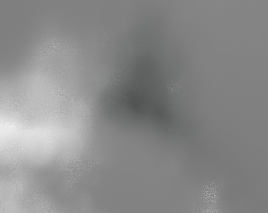
\includegraphics[width=4cm, height=3cm]{media/detail-factor-0.1.png}
    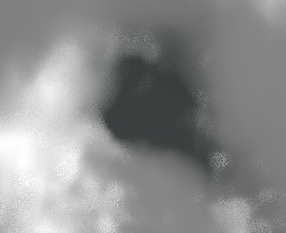
\includegraphics[width=4cm, height=3cm]{media/detail-factor-0.2.png}
    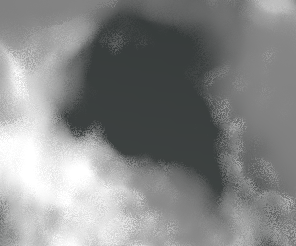
\includegraphics[width=4cm, height=3cm]{media/detail-factor-0.3.png}
    \caption{Detailfaktor - 0.0, 0.1, 0.2, 0.3}
    \label{fig:detail-factor}
\end{figure}

\subsubsection{Height Gradient}
Abbildung \ref{fig:height-gradient} zeigt das Ergebnis zwei verschiedener Paare an minimalen und maximalen Gradientenwerten für den Height Gradient aus Algorithmus \ref{alg:density}.

\begin{figure}[H]
    \centering
    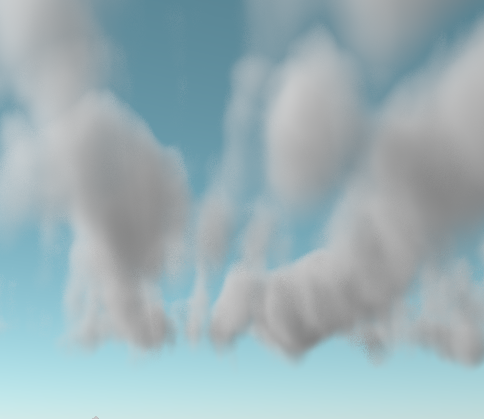
\includegraphics[width=4cm, height=3cm]{media/hg-low.png}
    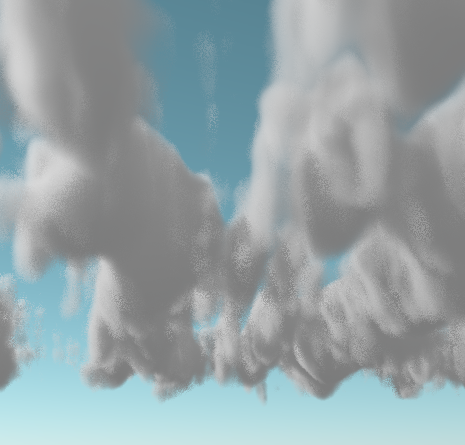
\includegraphics[width=4cm, height=3cm]{media/hg-high.png}
    \caption{Height Gradient - [0.1, 0.3], [0.7, 1.0]}
    \label{fig:height-gradient}
\end{figure}

\subsubsection{Ambient Gradient}
Abbildung \ref{fig:ambient-gradient} zeigt das Ergebnis zwei verschiedener Paare an minimalen und maximalen Gradientenwerten für den Ambient Gradient aus Algorithmus \ref{alg:lighting}.

\begin{figure}[H]
    \centering
    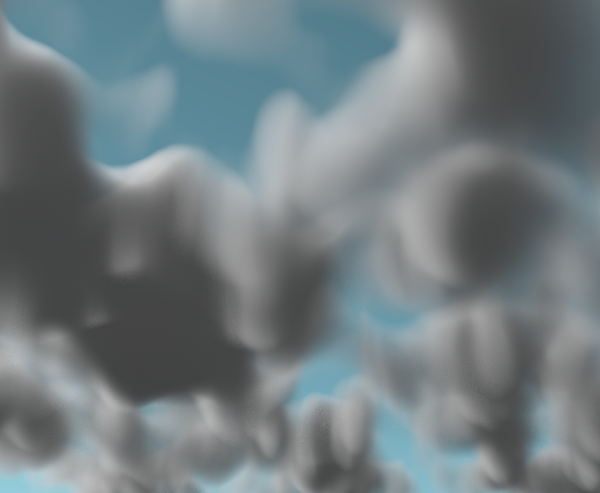
\includegraphics[width=4cm, height=3cm]{media/ag-low.png}
    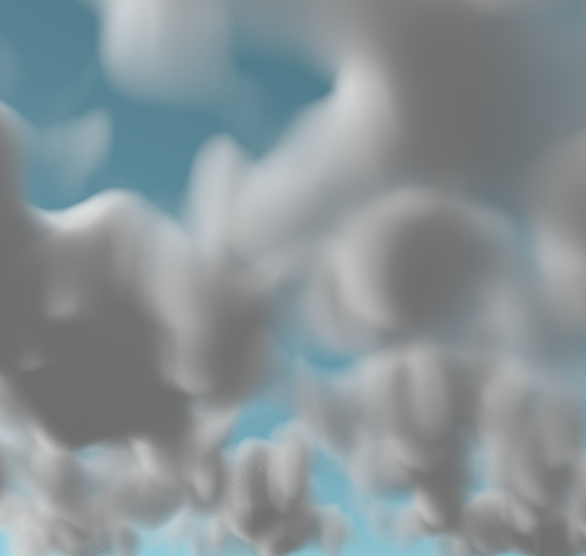
\includegraphics[width=4cm, height=3cm]{media/ag-high.png}
    \caption{Ambient Gradient - [0.15, 0.25], [0.5, 0.6]}
    \label{fig:ambient-gradient}
\end{figure}

\subsubsection{Empfehlung}
Im Allgemeinen sollten nicht weniger als 32 Primär Samples pro Pixel generiert werden, da sonst Artefakte deutlich sichtbar werden, wie in Abbildung \ref{fig:1st-sample} zu sehen ist. Weiterhin sollten mindestens 3 (am besten 4) Sekundär Samples verwendet werden. In Abbildung \ref{fig:2nd-sample} ist zu sehen, dass die Sekundär Samples den Wolken Tiefe verleihen. Der Jitteringfaktor sollte auf $ 1.0 $ gesetzt werden, da das Rauschen meist weniger auffällt als das Aliasing. Die Einstellung des Dichte Schwellwert, des Dichtefaktors, des Height Gradienten und des Ambient Gradienten sind abhängig von der angestrebten Wolkenart.

\subsection{Performanz}
Im folgenden Abschnitt wird auf die Performanz unter verschiedenen Optimierungen eingegangen. Die Werte wurden auf einem System mit einem AMD Ryzen 7 3700x (Release 2019) Prozessor und einer Nvidia GTX 970 (Release 2014) Grafikkarte gemessen. Der Renderer wurde mithilfe der Vulkan API implementiert.

Tabellen \ref{tab:perf_1} und \ref{tab:perf_2} zeigen die Performanz des Renderers in Bildern pro Sekunde. Die horizontalen Einträge unterscheiden sich in der Anzahl der Primär Samples und die vertikalen Einträge unterscheiden sich in der Anzahl der Sekundär Samples. Die unterschiedlichen Werte der vier Tabellen resultiert aus den Kombinationen aus Render Target Größe und dem Verwenden von Low Transmittance Early Exit mit dem Schwellwert $ 0.01 $.

\begin{table}[H]
\centering
\resizebox{\columnwidth}{!}{%}
    \begin{tabular}{|c|c|c|c|c|}
          \hline
        - & 16 & 32 & 48 & 64\\
        \hline
        1 & 47 & 29 & 21 & 10\\
        \hline
        2 & 43 & 26 & 19 & 10\\
        \hline
        3 & 41 & 23 & 14 & 6\\
        \hline
        4 & 39 & 23 & 13 & 6\\
        \hline
    \end{tabular}
    
    \begin{tabular}{|c|c|c|c|c|}
        \hline
        - & 16 & 32 & 48 & 64\\
        \hline
        1 & 43 & 26 & 19 & 8\\
        \hline
        2 & 39 & 23 & 18 & 8\\
        \hline
        3 & 37 & 21 & 13 & 6\\
        \hline
        4 & 34 & 21 & 12 & 6\\
        \hline
    \end{tabular}}
\caption{1920 x 1017 - Mit und ohne Early Exit}
\label{tab:perf_1}
\end{table}

\begin{table}[H]
\centering
\resizebox{\columnwidth}{!}{%}
    \begin{tabular}{|c|c|c|c|c|}
        \hline
        - & 16 & 32 & 48 & 64\\
        \hline
        1 & 121 & 72 & 55 & 30\\
        \hline
        2 & 110 & 65 & 50 & 30\\
        \hline
        3 & 105 & 56 & 39 & 23\\
        \hline
        4 &  98 & 55 & 36 & 20\\
        \hline
    \end{tabular}
    
    \begin{tabular}{|c|c|c|c|c|}
        \hline
        - & 16 & 32 & 48 & 64\\
        \hline
        1 & 112 & 64 & 50 & 26\\
        \hline
        2 & 102 & 57 & 45 & 26\\
        \hline
        3 &  94 & 50 & 34 & 20\\
        \hline
        4 &  88 & 50 & 32 & 18\\
        \hline
    \end{tabular}}
\caption{800 x 600 - Mit und ohne Early Exit}
\label{tab:perf_2}
\end{table}

Die Messungen zeigen, dass das Verwenden von Low Transmittance Early Exit die Performanz um bis zu $ 25\% $ steigern kann. Das Vierteln ($ 4.068 = \frac{1920 \cdot 1017}{800 \cdot 600} $) der Render Target Größe führt zu einer Verdoppelung bis Verdreifachung der Bilder pro Sekunde.

\subsection{Gezieltes Rendern von Wolkenarten}
Im Folgenden wird beschrieben, wie die behandelten Parameter und Texturen genutzt werden können, um typische Wolkenformen zu rendern.

\subsubsection{Stratus}
Wolken vom Typ Stratus bilden eine ebene Wolkenschicht mit wenigen Lücken und sind niedrig positioniert. Dieser Effekt lässt sich durch folgende Parameter erzielen.

\begin{enumerate}
    \item uniform verteilter Altitude Kanal in der Weather Textur
    \item geringe Eintrittshöhe des Volumens (hier $ 1500 $)
    \item geringer Detailfaktor (hier $ 0.05 $)
    \item hoher Ambient Gradient min ($ 0.8 $) und max ($ 1.0 $)
\end{enumerate}

\begin{figure}[H]
    \centering
    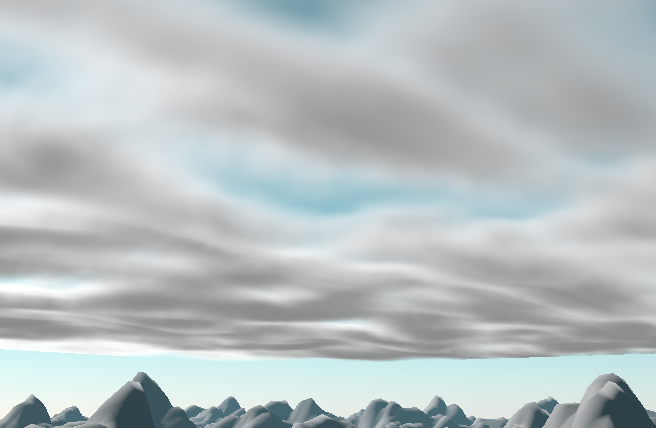
\includegraphics[width=8cm]{media/stratus.png}
    \caption{Stratus Wolken Render}
    \label{fig:stratus}
\end{figure}

\subsubsection{Stratonimbus}
Wolken vom Typ Stratonimbus sind dunkel aufgrund des Niederschlags (nimbus) und bilden eine Wolkenschicht mit wenigen Lücken (stratus), wie Abbildung \ref{fig:stratonimbus} zeigt. Die folgenden Parameter erzielen diesen Effekt.

\begin{enumerate}
    \item uniform verteilter Altitude Kanal in der Weather Textur
    \item geringe Eintrittshöhe des Volumens (hier $ 1500 $)
    \item geringer Detailfaktor (hier $ 0.05 $)
    \item niedriger Ambient Gradient min ($ 0.1 $) und max ($ 0.3 $)
\end{enumerate}

\begin{figure}[H]
    \centering
    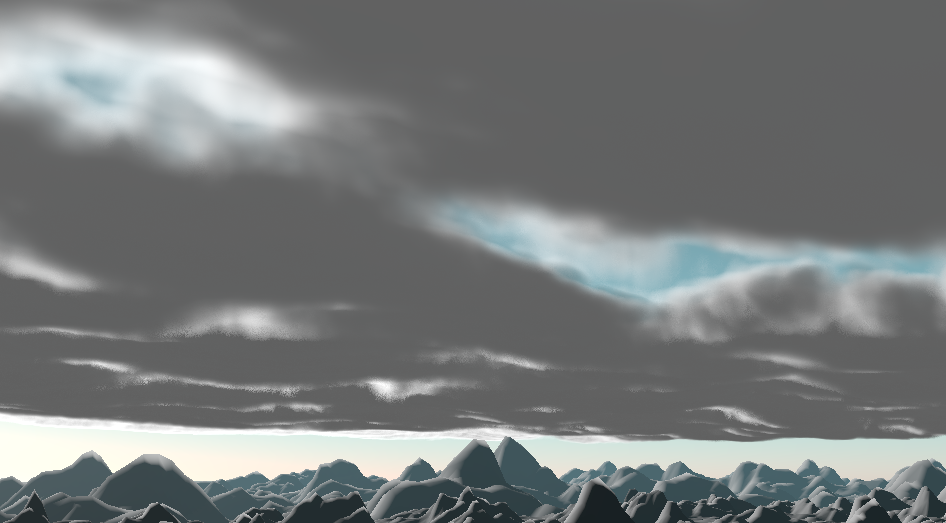
\includegraphics[width=8cm]{media/stratonimbus.png}
    \caption{Stratonimbus Wolken Render}
    \label{fig:stratonimbus}
\end{figure}

\subsubsection{Cumulus}
Cumulus Wolken sind wie vereinzelte Haufen verteilt. Um diesen Effekt zu erzielen, werden folgende Parameter und Textureigenschaften gewählt.

\begin{enumerate}
    \item der Coverage Kanal der Weather Textur sollte viele nicht zusammenhängende Flecken haben (hier durch Worley Noise)
    \item hoher Detailfaktor (hier $ 0.5 $)
    \item hoher Detail Schwellwert (hier $ 1.0 $)
\end{enumerate}

\begin{figure}[H]
    \centering
    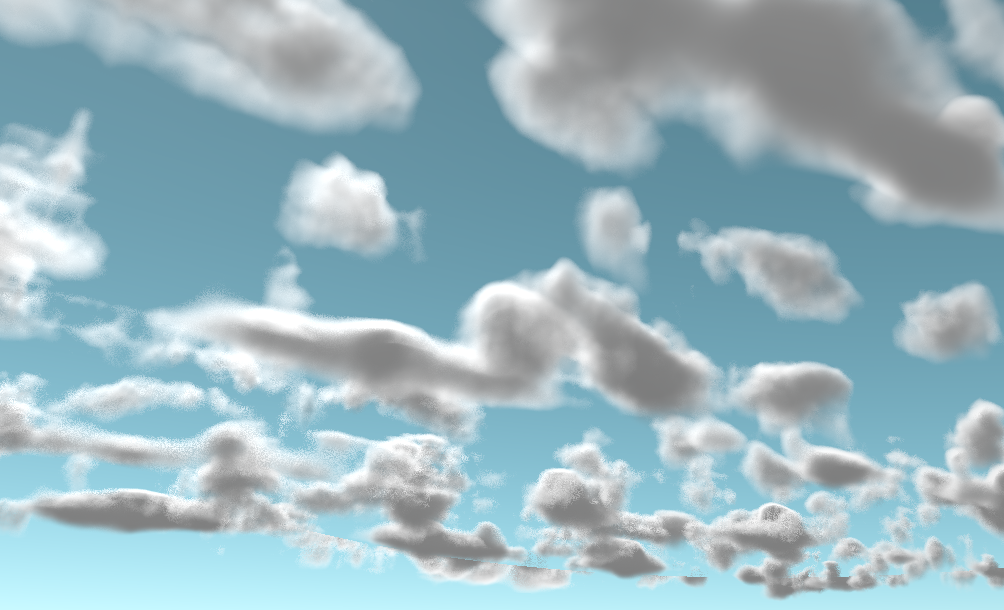
\includegraphics[width=8cm]{media/cumulus.png}
    \caption{Cumulus Wolke Render}
    \label{fig:cumulus}
\end{figure}

\section{Fazit}
\label{sec:conclusion}

Wie die Ergebnisse aus Sektion \ref{sec:evaluation} zeigen, können Wolken auf einem Render Target von 800 x 600 mit 48 Primär Samples und 4 Sekundär Samples mit  über 30 Bildern pro Sekunde gerendert werden. Bemerkenswert ist, dass dieses Ergebnis auf Grafikhardware aus dem Jahr 2014 erzielt wurde. Mit einer Kombination aus weiteren Optimierungen und moderner Grafikhardware kann unser Ansatz verwendet werden, um Wolken in Echtzeit mit komplexer Szenengeometrie zu rendern.

Neben den bereits genannten Ansätzen wie eine runde Atmosphäre, Temporal Upsampling und High Transmittance Early Exit bieten sich weitere Weiterentwicklungen unseres Renderers an. Dazu gehören eine genauere Wechselwirkung zwischen Geometrie und Wolken, da diese gegenseitige Schatten werfen können \cite{Högfeldt16}. Diese Schatten können in Kombination mit sich durch Wind bewegenden Wolken die Szene dynamischer gestalten, da sich die Lichtverhältnisse so öfter ändern. Wie in Sektion \ref{sec:evaluation} gezeigt wird, kann durch geschickte Wahl der Parameter gezielt eine Wolkevariante gerendert werden. In der Realität kommen häufig mehrere Wolkentypen gleichzeitig vor, unter anderem aufgrund unterschiedlicher Höhen. Högfeldt \cite{Högfeldt16} löst diesen Sachverhalt, durch das Verwenden von verschiedenen Schichten. Diese Methode lässt sich auch auf unseren Renderer anwenden, indem mehrere Instanzen an Volumen und Parametern gleichzeitig gerendert werden.

\clearpage


\printbibliography

\end{document}
